\chapter{Magnetic separation configuration}\label{ch:magneticSeparationConfiguration}
%\emph{Simulation software such as ANSYS Maxwell makes it possible to simulate complex magnet geometries, without the need of time consuming and laborious experimental work. This chapter will look at two new magnet geometries which improve the existing magnetic configurations for continuous separation.}

\section{Introduction}\label{sec:introduction}
A key objective was to design a novel magnet configuration that would enable continuous separation of magnetic particles of variable susceptibility while reducing particle interactions with the side walls of the microfluidic channel. 

As seen in Chapter~\ref{ch:introduction}, magnetic separation configurations typically use a strong rare-earth magnet or an electromagnet in close proximity to the channel to attract and repel paramagnetic and diamagnetic particles, respectively. In either case, the force is always unidirectional; meaning all particles are either attracted or repelled from the magnet. The magnet configurations presented here have the ability to attract and repel superparamagnetic particles.

\section{Magnet configurations}\label{sec:magnetConfiguration}
The two magnet configurations incorporate two or four bar magnets, which are placed at the side of the microfluidic channel, as depicted in Figure~\ref{fig:magnetConfigurations}. The resulting forces on magnetic particles applied to their separation process is novel. Both configurations use N42 Neodymium magnets of dimension $20$ mm $\times$ $6$ mm $\times$ $1.5$ mm (First4Magnets$^\textsuperscript{\textregistered}$,UK), which can be conveniently machined to change their shape. The two geometries will be referred to as Double Magnet and Quadrupole configuration throughout this thesis. 
\begin{figure}[tb]
\centering
	\begin{subfigure}[b]{0.48\textwidth}
		\includegraphics[width=\textwidth]{img/chapters/chapter_6_magnet_configurations/magnetConfigurationDoubleMagnet.pdf}
		\caption{Double Magnet configuration}
		\label{fig:double}
    \end{subfigure}
    \hfill
	\begin{subfigure}[b]{0.48\textwidth}
		\includegraphics[width=\textwidth]{img/chapters/chapter_6_magnet_configurations/magnetConfigurationQuadrupoleMagnet.pdf}
		\caption{Quadrupole configuration}
		\label{fig:quadrupole}
	\end{subfigure}
\caption[3D Schematic of the magnet configurations]{3D schematic of the two magnet configurations used in this thesis. (a) shows the Double Magnet configuration and (b) the Quadrupole configuration and how the magnets are placed around the microfluidic channel. The dimensions of the magnets are $20$ mm $\times$ $6$ mm $\times$ $1.5$ mm.}%
\label{fig:magnetConfigurations}
\end{figure}
All numerical results for the magnetic $\mathbf{B}$ field and the magnetophoretic driving force were obtained by using the previously described techniques for FEM and smoothing.  

\subsection{Double Magnet configuration}\label{subsec:doubleMagnetConfiguration}
The Double Magnet configuration shown in Figure~\ref{fig:double} is the most basic geometry used here. Two magnets are placed on top of each other in an attractive configuration, with both magnetizations pointing in the same direction. The microfluidic channel is located along the $x$ axis to the right of the magnet configuration as depicted in Figure~\ref{fig:doubleMagnetConfigurationSchematic}. 
\begin{figure}[htb]
\centering
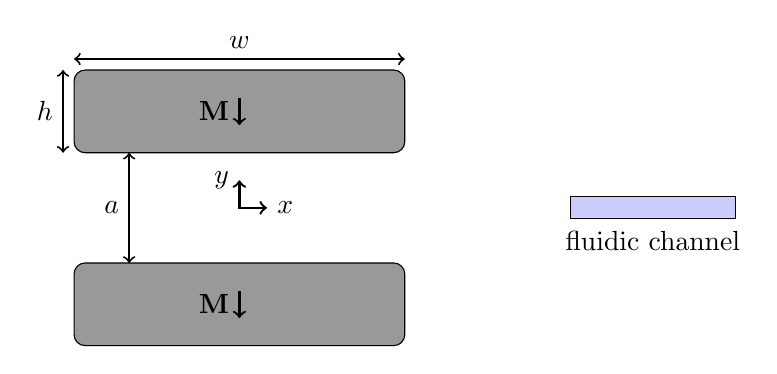
\begin{tikzpicture}[scale=0.7]
	\filldraw[rounded corners, fill=black!40!white, draw=black] (-9,1) rectangle (-3,2.5);
	\filldraw[rounded corners, fill=black!40!white, draw=black] (-9,-1) rectangle (-3,-2.5);	
	\filldraw[fill=blue!20!white, draw=black] (0,-0.2) rectangle (3,0.2);	
	\node[thick] at (1.5,-0.6) {fluidic channel};
					
	\draw[line width=0.3mm,<->] (-6,0.5) node[anchor=east] {$y$} -- (-6,0) -- (-5.5,0) node[anchor=west] {$x$};

	\draw[thick,->] (-6,2) -- node[thick,anchor=east]{$\mathbf{M}$} (-6,1.5);
	\draw[thick,->] (-6,-1.5) -- node[thick,anchor=east]{$\mathbf{M}$} (-6,-2);
	\draw[line width=0.25mm,<->] (-9,2.7) -- node[anchor=south]{$w$} (-3,2.7);
	\draw[line width=0.25mm,<->] (-9.2,1) -- node[anchor=east]{$h$} (-9.2,2.5);
	\draw[line width=0.25mm,<->] (-8,-1) -- node[anchor=east]{$a$} (-8,1);
\end{tikzpicture}
\caption[2D diagram of the Double Magnet configuration]{2D slice diagram ($z=0$) of the Double Magnet configuration used to generate the external magnetic field for separation. The rectangular permanent magnets (grey) are set up in attraction, with the magnetization in the negative $y$ direction as indicated by the magnetization vector $\mathbf{M}$. The parameters $w$, $h$ and $a$ describe the width, the height (thickness) and the separation of the two magnets. The microfluidic channel is located (light blue) to the right of the magnet configuration. The schematic is not drawn to scale.}
\label{fig:doubleMagnetConfigurationSchematic}
\end{figure}
The three geometric parameters of the system and their ratios, shown in Figure~\ref{fig:doubleMagnetConfigurationSchematic}, are used to quantify the distribution of the magnetic field and force; height $h$ and width $w$ of the magnets and their vertical spacing $a$. The impact of varying two ratios is studied here: $h/w$ (aspect ratio) and $a/w$ (relative gap).

As a conservative magnetic field ($\mathbf{\nabla} \cdot \mathbf{B} = 0$), an intrinsic property of the magnetic flux density is the formation of complete closed flux loops around the magnet. The spatial distribution of the flux loops is a function of the number, position and magnetization orientation of the magnets, and represents the vector field of the magnetic flux density $\mathbf{B}$. In Figure~\ref{fig:magneticFluxDensityDoubleMagnetConfiguration} the magnetic flux density and its field lines of the Double Magnet configuration is shown. The field lines form loops around each individual magnet as well as around the whole magnet configuration. Due to the field lines looping around each individual magnet their superposition results in a region where magnetic flux density is zero ($|\mathbf{B}|=0$ at point \circled{2} in Figure~\ref{fig:magneticFluxDensityDoubleMagnetConfiguration}) because of their opposing direction. Also, local flux density extrema (maximum or minimum) are generated where $\nabla|\mathbf{B}|=0$ (point \circled{1} and point \circled{3} in Figure~\ref{fig:magneticFluxDensityDoubleMagnetConfiguration}).
\begin{figure}[htb]
   \centering
   \includegraphics[width=0.7\textwidth]{img/chapters/chapter_6_magnet_configurations/doubleMagnetConfigurationFluxDensity.pdf}
   \caption[Simulated vector field and flux density of the Double Magnet configuration]{Modelling of the magnetic flux density $\mathbf{B}$ of the Double Magnet configuration in the plane $z=0$ when the vertical separation $a=3$ mm. The positions where the magnetic driving force is zero, and thus magnetic beads experience no horizontal magnetic force, are indicated by the points \circled{1}, \circled{2} and \circled{3}.}
   \label{fig:magneticFluxDensityDoubleMagnetConfiguration}
\end{figure}
Magnetic particles will experience no force in a magnetic field if either the magnitude of the flux density is zero ($|\mathbf{B}|=0$) or there is no field gradient ($\nabla|\mathbf{B}|=0$), i.e. they are in a region of zero or a local minimum in magnetic energy density. In Figure~\ref{fig:magneticFluxDensityAndFluxGradientDoubleMagnetConfiguration} the magnetic flux density of the Double Magnet configuration is plotted along the $x$ axis, starting at $x=y=z=0$. Three points are indicted in Figure~\ref{fig:magneticFluxDensityAndFluxGradientDoubleMagnetConfiguration} where these conditions are met. Such points where no horizontal magnetic force is exerted are useful to trap or gather magnetic beads.
\begin{figure}[htb]
   \centering
   \begin{subfigure}[b]{0.48\textwidth}
   \includegraphics[width=\textwidth]{img/chapters/chapter_6_magnet_configurations/doubleMagnetMagneticFieldFlux.pdf}
   \caption{}
   \label{fig:doubleMagnetMagneticFieldFlux}
   \end{subfigure}
   \hfill
   \begin{subfigure}[b]{0.48\textwidth}
   \includegraphics[width=\textwidth]{img/chapters/chapter_6_magnet_configurations/doubleMagnetMagneticFieldFluxGradient.pdf}
   \caption{}
   \label{fig:doubleMagnetMagneticFieldFluxGradient}
   \end{subfigure}
   \caption[Magnetic flux density and flux density gradient of the Double Magnet configuration]{(a) Magnetic flux density and (b) flux density gradient of the Double Magnet configuration with a vertical separation $a=3$ mm. The magnetic flux density is simulated and measured along the $x$ axis, as indicated in the inset, starting at $x=y=z=0$ mm. Due to symmetry, only the positive $x$ axis is shown. Points \circled{1}, \circled{2} and \circled{3} indicate the positions where beads experience no horizontal magnetic force.}
   \label{fig:magneticFluxDensityAndFluxGradientDoubleMagnetConfiguration}
\end{figure}
One location, where particles experience no force is in the exact centre of the Double Magnet configuration for $x=0$, labelled as \circled{1} in Figure~\ref{fig:magneticFluxDensityDoubleMagnetConfiguration} and Figure~\ref{fig:magneticFluxDensityAndFluxGradientDoubleMagnetConfiguration}. This point has already been exploited to trap magnetic beads~\cite{Gassner2009}. At \circled{2}, where $|\mathbf{B}|=0$, beads will not gather due to the gradient and thus should be avoided if the goal is to accumulate beads. The gathering point where $\nabla|\mathbf{B}|=0$, point \circled{3}, on the other hand, appears to be a stable gathering point and will be further investigated in this study. 

The stable gathering point at \circled{3} is important for trapping and manipulating magnetic beads because any small disturbance to a bead's position will result in a restorative force to return it to the same point. This is best illustrated when plotting the magnetic force along the $x$ axis, as shown in Figure~\ref{fig:doubleMagnetConfiguraitonMagneticDrivingForce}. The change in sign of the force results in regions where particles either experience an attractive or repulsive force. The direction in which superparamagnetic particles are moving, depending on their position, is also schematically illustrated in Figure~\ref{fig:doubleMagnetConfigurationBeadMovementSchematic}.
\begin{figure}[htb]
   \centering
   \begin{subfigure}[b]{0.48\textwidth}
   \includegraphics[width=\textwidth]{img/chapters/chapter_6_magnet_configurations/doubleMagnetMagneticForce.pdf}
   \caption{}
   \label{fig:doubleMagnetConfiguraitonMagneticDrivingForce}
   \end{subfigure}
   \hfill
   \begin{subfigure}[b]{0.48\textwidth}
   \includegraphics[width=\textwidth]{img/chapters/chapter_6_magnet_configurations/doubleMagnetConfigurationFluxDensityParticleMovementUnited.pdf}
   \caption{}
   \label{fig:doubleMagnetConfigurationBeadMovementSchematic}
   \end{subfigure}
   \caption[Magnetic driving force of the Double Magnet configuration on a superparamagnetic bead]{(a) Magnetic force on a single Dynabead M270  bead along the $x$-axis when being exposed to the Double Magnet configuration. The arrows indicate the region where the particle experiences an attractive (red arrow) or a repulsive force (green arrow). The magnet configuration parameters are assumed to be $6$ mm, $1.5$ mm and $2.6$ mm for the magnet width, magnet height and vertical spacing, respectively. (b) Schematic of the direction of movement of superparamagnetic beads when being exposed to the magnetic field of the Double Magnet configuration.}
   \label{fig:doubleMagnetConfigurationMagneticDrivingForceAndBeadMovementSchematic}
\end{figure}
In the following sections, different geometry parameters of the Double Magnet configuration (see Figure~\ref{fig:doubleMagnetConfigurationSchematic}) and their influence on the gathering point outside of the magnet, point \circled{3}, will be investigated.

\subsubsection{Effects of magnet aspect ratio}\label{subsubsec:effectsOfMagnetAspectRatio}
For the Double Magnet configuration, Figure~\ref{fig:doubleMagnetConfigurationMagneticDrivingForceAndFluxDensityForDifferentAspectRatio} shows the  simulated magnetophoretic driving force along the $x$ axis, for different aspect ratios $h/w$ ranging from $0.25$ to $3$. In this particular study, the magnet width $w$ and vertical separation $a$ are kept constant at $6$ mm and $2$ mm, respectively, while the thickness, $h$, of the two magnets is varied keeping $h$ the same for both magnets. 

\begin{figure}[htb]
	\centering
	\includegraphics[width=\textwidth]{img/chapters/chapter_6_magnet_configurations/doubleMagnetConfigurationMagneticDrivingForceForDifferentAspectRatio.pdf}
\caption[Magnetophoretic driving force of the Double Magnet configuration for different magnet aspect ratio]{Magnetophoretic driving force of the Double Magnet configuration along the $x$ axis for different aspect ratio $h/w$ ranging from $0.25-3$. The shaded area indicates the overlap of the magnets along the $x$ direction. The inset shows the line along which the magnetophoretic driving force is simulated. When the force is positive a magnetic bead will be pushed away from the magnets (to the right) and toward the magnets when negative. This change from right to left establishes the stable gathering points. Note that a larger aspect ratio moves the gathering point away from the magnet configuration.}
\label{fig:doubleMagnetConfigurationMagneticDrivingForceAndFluxDensityForDifferentAspectRatio}
\end{figure}

From Figure~\ref{fig:doubleMagnetConfigurationMagneticDrivingForceAndFluxDensityForDifferentAspectRatio} it can be seen that the gathering point \circled{3} moves further away from the magnets with increasing aspect ratio. This also lowers the magnetophoretic driving force in the vicinity of the gathering point. At higher aspect ratios ($h/w \geq 3$), the gathering point disappears because the magnet separation compared to their height becomes insignificant and the Double Magnet configuration can be regarded as approaching a single magnet.  

The setup described in Section~\ref{sec:equilibriumPositionExperiment} was used to verify by experiment the behaviour of the gathering points for different aspect ratios (see Section~\ref{subsec:magnetHeightVariation}). Figure~\ref{fig:stableGatheringPointAspectRatio} shows the experimental results revealing how the gathering position moves along the $x$ axis away from the magnets when the aspect ratio is increased for different magnetic bead types. The experimental observations affirm the simulated results and it appears that the gathering position and magnet aspect ratio have a linear relationship over the range investigated.

\begin{figure}[htb]
\centering
	\includegraphics[width=0.7\textwidth]{img/chapters/chapter_6_magnet_configurations/doubleMagnetConfigurationGatheringPointAspectRatio_particles.eps}
\caption[Observed behaviour of position of the static gathering point as a function of the magnet aspect ratio]{Observed behaviour of the position of the static gathering point outside of the Double Magnet configuration as a function of the magnet aspect ratio $h/w$ while keeping $a=2$ mm. The data is collected by experiment. The error bars are computed from different measurements of bead suspension of the same bead type but different bead concentrations.}
\label{fig:stableGatheringPointAspectRatio}
\end{figure}

\subsubsection{Effects of vertical separation between magnets}\label{subsubsec:effectsOfVerticalSeparationBetweenMagnets}
Figure~\ref{fig:doubleMagnetConfigurationMagneticDrivingForceAndFluxDensityForDifferentSeparationRatio} shows the evolution of the magnetophoretic driving force, as a function of the relative gap $a/w$. The aspect ratio $h/w$ of the magnet is kept constant at $0.25$ ($w=6$ mm and $h=1.5$ mm) and only the separation $a$ is varied.

\begin{figure}[htb]
	\centering
	\includegraphics[width=\textwidth]{img/chapters/chapter_6_magnet_configurations/doubleMagnetConfigurationMagneticDrivingForceForDifferentSeparationRatio.pdf}
\caption[Magnetophoretic driving force of the Double Magnet configuration for different separation ratio]{Magnetophoretic driving force of the Double Magnet configuration along the $x$ axis at $y=0$ for different separation ratios $a/w$ ranging from $0.2$ to $1$. The shaded area indicates the region between the magnets along the $x$ direction. Increasing the separation between the magnets moves the gathering point away from the magnets and reduces the magnetophoretic driving force.}
\label{fig:doubleMagnetConfigurationMagneticDrivingForceAndFluxDensityForDifferentSeparationRatio}
\end{figure}

The position of the stable gathering point is again moved along the $x$ axis away from the Double Magnet configuration when the vertical separation between the two magnets is increased. This can be better seen in the magnified section in Figure~\ref{fig:doubleMagnetConfigurationMagneticDrivingForceAndFluxDensityForDifferentSeparationRatio} by the moving intercept of the curves with the force $=0$ line. Increasing the magnet separation results in both a lower magnetic flux magnitude and gradient outside of the magnets. This in turn leads to a lower magnitude and gradient of the magnetophoretic driving force in and around the particle gathering region and thus the \textit{separating power} will be decreased.

Experimental observation of the gathering point for different magnetic bead types again reveals a linear relationship between the relative vertical gap, $a/w$, and the gathering point position, as shown in Figure~\ref{fig:stableGatheringPointSeparationRatioParticle}. The gathering point of all bead types increases as the relative gap between the magnets increases, and the experimental values are a good fit to the positions determined by the model. 

\begin{figure}[htb]
\centering
	\includegraphics[width=0.7\textwidth]{img/chapters/chapter_6_magnet_configurations/doubleMagnetConfigurationGatheringPointSeparationRatio_color.eps}
\caption[Observed gathering position as a function of the magnet separation ratio for different particle types]{Experimental results of the observed gathering positions for different magnetic bead types and vertical separation ratios $a/w$. The error bars for each particle type are calculated from repeated measurements with different bead concentrations.}
\label{fig:stableGatheringPointSeparationRatioParticle}
\end{figure}

Figure~\ref{fig:stableGatheringPointSeparationRatioConcentration} shows the result of a similar experiment to that presented in Figure~\ref{fig:stableGatheringPointSeparationRatioParticle}, however, only one bead type (Dynabeads M270) has been used for significantly different concentrations. Based on Figure~\ref{fig:stableGatheringPointSeparationRatioConcentration}, changing the concentration appears to have no effect on the position of the stable gathering position when varying the relative magnet separation ratio.

\begin{figure}[htb]
\centering
	\includegraphics[width=0.7\textwidth]{img/chapters/chapter_6_magnet_configurations/doubleMagnetConfigurationGatheringPointSeparationRatio_concentration.eps}
\caption[Gathering positions as a function of the magnet separation ratio for different particle suspension concentration]{Experimental observations of the gathering positions at different vertical separation ratios $a/w$ for Dynabeads M270 at three particle suspension concentrations.}
\label{fig:stableGatheringPointSeparationRatioConcentration}
\end{figure}

\subsubsection{Effects of tapered magnets}\label{subsubsec:effectsOfTaperedMagnets}
As seen previously in Section~\ref{subsubsec:effectsOfMagnetAspectRatio} and Section~\ref{subsubsec:effectsOfVerticalSeparationBetweenMagnets}, changing the thickness or the vertical separation between the magnets, alters the strength of the magnetophoretic driving force as well as the position of the static gathering point. By tapering the magnets, these two effects can be combined. Tapering the magnets could also be used to gradually reduce the magnetophoretic driving force at the tail-end of the magnets in order to gently release particles into an exit flow that would otherwise be at risk of being trapped.

The two magnet shapes considered here that incorporate a taper are shown in Figure~\ref{fig:taperedMagnetSchematic}. The taper is either on the inner faces (Figure~\ref{fig:taperInner}) or the outer faces (Figure~\ref{fig:taperOuter}), beginning halfway along the length of the magnets. In these diagrams, the channel will flow from left to right ($z$ direction) whilst the magnetic force on the particles is predominantly in the $x$ direction. Different tapering angles, $\theta$, are modelled assuming the starting magnet to be a N42 Neodymium magnet with dimensions $20$ mm $\times$ $6$ mm $\times$ $1.5$ mm. The vertical separation is set to $a=2.6$ mm. There are many tapered geometries that could be explored, but these simple structures have been selected for evaluation purposes. 

\begin{figure}[htb]
\centering
	\begin{subfigure}[b]{0.48\textwidth}
	\centering
	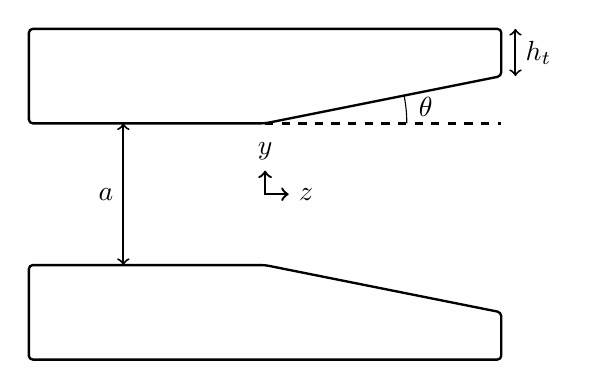
\begin{tikzpicture}[scale=0.6]
		\draw [line width=0.3mm, rounded corners=0.5mm] (0,1.5)--(-5,1.5)--(-5,3.5)--(5,3.5)--(5,2.5)-- cycle;	
		\draw [line width=0.3mm, rounded corners=0.5mm] (0,-1.5)--(-5,-1.5)--(-5,-3.5)--(5,-3.5)--(5,-2.5)-- cycle;			
		\draw [line width=0.3mm,<->] (0,0.5) node[anchor=south] {$y$} -- (0,0) -- (0.5,0) node[anchor=west] {$z$};
		\draw [line width=0.25mm,<->] (-3,-1.5) -- node[anchor=east]{$a$} (-3,1.5);
		\draw [line width=0.25mm,<->] (5.3,2.5) -- node[anchor=west]{$h_{t}$} (5.3,3.5);

		\draw [line width=0.3mm,dashed] (0,1.5)--(5,1.5); 
		\draw (3,1.5) arc (0:11:3);
		\node[] at (3.4,1.85) {$\theta$};
	\end{tikzpicture}
	\caption{Inner taper}
    \label{fig:taperInner}
    \end{subfigure}
    \hfill
	\begin{subfigure}[b]{0.48\textwidth}
	\centering
	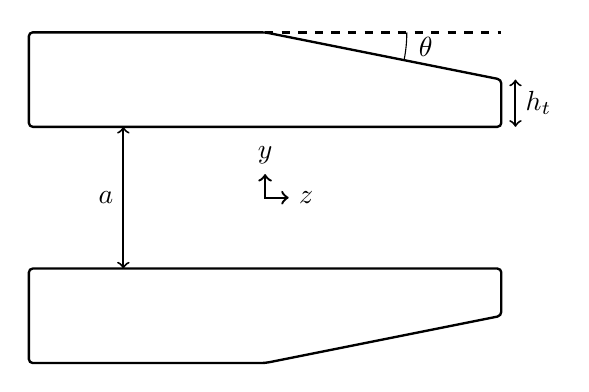
\begin{tikzpicture}[scale=0.6]
		\draw [line width=0.3mm, rounded corners=0.5mm] (-5,1.5)--(-5,3.5)--(0,3.5)--(5,2.5)--(5,1.5) -- cycle;	
		\draw [line width=0.3mm, rounded corners=0.5mm] (-5,-1.5)--(-5,-3.5)--(0,-3.5)--(5,-2.5)--(5,-1.5) -- cycle;	
		\draw[line width=0.3mm,<->] (0,0.5) node[anchor=south] {$y$} -- (0,0) -- (0.5,0) node[anchor=west] {$z$};
		\draw[line width=0.25mm,<->] (-3,-1.5) -- node[anchor=east]{$a$} (-3,1.5);	
		\draw [line width=0.25mm,<->] (5.3,1.5) -- node[anchor=west]{$h_{t}$} (5.3,2.5);

		\draw [line width=0.3mm,dashed] (0,3.5)--(5,3.5); 
		\draw (3,3.5) arc (0:-11:3);
		\node[] at (3.4,3.2) {$\theta$};
	\end{tikzpicture}
	\caption{Outer taper}
	\label{fig:taperOuter}
	\end{subfigure}
\caption[Diagrams of the tapered magnet configurations]{Diagrams of the tapered magnet configurations: (a) inner taper (b) outer taper. The taper begins halfway along the length of the magnets and finishes at half the non-tapered thickness of the magnets. Schematic is not drawn to scale.}
\label{fig:taperedMagnetSchematic}
\end{figure}

In Figure~\ref{fig:taperedMagnetDrivingForce} it can be seen that for both taper options, a larger tapering angle results in a lower magnetophoretic driving force around the static gathering position. This effect is more pronounced for the magnets which are tapered on the inner faces. This is due to the fact that the magnet separation increases with the taper. 

The particle gathering positions are also affected by the taper, either pushing the gathering point out for magnets with inner tapers or pulling the gathering point in for magnets with outer tapers (see magnified section in Figure~\ref{fig:taperedMagnetDrivingForce}).

\begin{figure}[htb!]
\centering
	\begin{subfigure}[b]{\textwidth}
		\centering
		\includegraphics[width=\textwidth]{img/chapters/chapter_6_magnet_configurations/doubleMagnetConfigurationMagneticDrivingForceInnerTaper.pdf}
	\caption{Inner taper}
    \label{fig:innterTaperDrivingForce}
    \end{subfigure}
    \begin{subfigure}[b]{\textwidth}
    	\centering
		\includegraphics[width=\textwidth]{img/chapters/chapter_6_magnet_configurations/doubleMagnetConfigurationMagneticDrivingForceOuterTaper.pdf}
	\caption{Outer taper}
    \label{fig:outerTaperDrivingForce}
	\end{subfigure}
\caption[Simulation of the magnetophoretic driving force for different magnet tapers]{Simulation of the magnetophoretic driving force for magnets with different angles of tapers. Taper angle is varied by changing the magnet thickness at the end of the taper between $h_{t}=0.75$ mm and $h_{t}=1.5$ mm. (a) Shows the magnetophoretic driving force when the magnets are tapered on the inside. (b) Shows the magnetophoretic driving force when the magnets are tapered on the outside. The magnets are simulated as N42 Neodymium magnets with original dimensions of $20$ mm $\times$ $6$ mm for length and width, respectively, and $1.5$ mm for non-tapered height.}
\label{fig:taperedMagnetDrivingForce}
\end{figure}

The inner taper configuration, shown in Figure~\ref{fig:taperInner}, has been experimentally evaluated (see Figure~\ref{fig:taperedMagnetGatheringPointExperiment}). There is a clear difference in the static gathering position between the non-tapered and the tapered half of the magnet faces. An observable monotonic increase in the gathering position as the magnets become thinner, as well as a reduction in the particle concentration, could be observed.

\begin{figure}[htb]
\centering
		\includegraphics[width=0.6\textwidth]{img/chapters/chapter_6_magnet_configurations/particleAgglomerationBandTaperTopView_color.pdf}
\caption[Static particle gathering band for tapered Double Magnet configuration]{Static particle gathering band for the Double Magnet configuration using two tapered N42 NdFeB magnets. The magnets' original dimensions were $20$ mm $\times$ $6$ mm $\times$ $1.5$ mm. The taper begins half way along the magnet and reduced the magnet thickness to half of its original thickness ($h_{t}\approx 0.75$ mm). There is an increase in the static equilibrium distance with decreasing magnet thickness.}
\label{fig:taperedMagnetGatheringPointExperiment}
\end{figure}

%\begin{figure}[htb]
%\centering
%	\begin{subfigure}[b]{0.48\textwidth}
%		\includegraphics[width=\textwidth]{img/chapters/chapter_6_magnet_configurations/particleAgglomerationBandTaperNo.pdf}
%    \label{fig:taperedMagnetExperiementNo}
%    \end{subfigure}
%    \hfill
%    \begin{subfigure}[b]{0.48\textwidth}
%	\includegraphics[width=\textwidth]{img/chapters/chapter_6_magnet_configurations/particleAgglomerationBandTaperYes.pdf}
%    \label{fig:taperedMagnetExperiementYes}
%    \end{subfigure}
%\caption[Static particle gathering band for tapered double magnet configuration]{Static particle gathering band for the double magnet configuration using two tapered $20 \times 6 \times 1.5$ mm N42 NdFeB magnets. a) Particle band along the non-tapered edge. b) Particle band along the tapered edge. There is a linear increase in the static equilibrium position with increasing magnet taper.}%
%\label{fig:taperedMagnetGatheringPointExperiment}
%\end{figure}

\subsection{Quadrupole configuration}\label{subsec:quadrupoleMagnetConfiguration}
A second Double Magnet can be added to create a Quadrupole configuration, where the microfluidic channel is assumed to be always in the centre of the geometry. A 2D schematic of the Quadrupole configuration is shown in Figure~\ref{fig:quadrupoleMagnetConfiguration}.

\begin{figure}[htb]
\centering
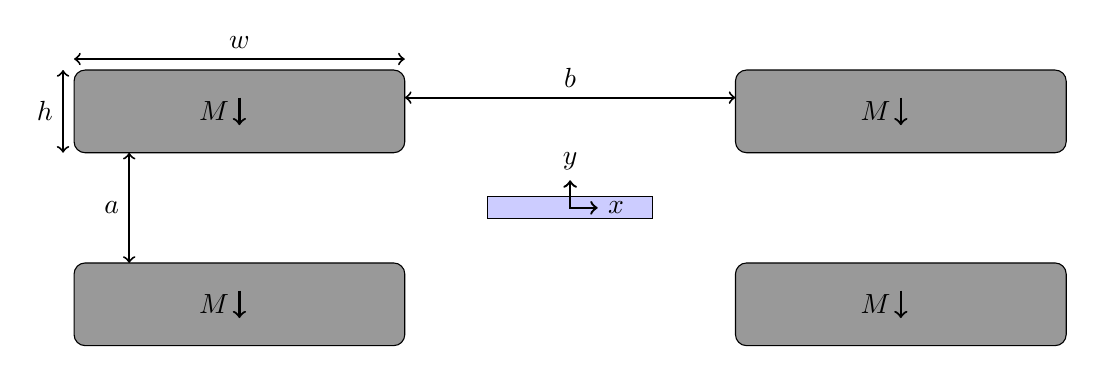
\begin{tikzpicture}[scale=0.7]
	\filldraw[rounded corners, fill=black!40!white, draw=black] (-9,1) rectangle (-3,2.5);
	\filldraw[rounded corners, fill=black!40!white, draw=black] (-9,-1) rectangle (-3,-2.5);	
	\draw[thick,->] (-6,2.0) -- node[thick,anchor=east]{$M$} (-6,1.5);
	\draw[thick,->] (-6,-1.5) -- node[thick,anchor=east]{$M$} (-6,-2.0);

	\filldraw[fill=blue!20!white, draw=black] (-1.5,-0.2) rectangle (1.5,0.2);					
	\filldraw[rounded corners, fill=black!40!white, draw=black] (9,1) rectangle (3,2.5);
	\filldraw[rounded corners, fill=black!40!white, draw=black] (9,-1) rectangle (3,-2.5);	
	\draw[thick,->] (6,2.0) -- node[thick,anchor=east]{$M$} (6,1.5);
	\draw[thick,->] (6,-1.5) -- node[thick,anchor=east]{$M$} (6,-2.0);
	
	\draw[line width=0.3mm,<->] (0,0.5) node[anchor=south] {$y$} -- (0,0) -- (0.5,0)
	 node[anchor=west] {$x$};
	 
	\draw[line width=0.25mm,<->] (-9,2.7) -- node[anchor=south]{$w$} (-3,2.7);
	\draw[line width=0.25mm,<->] (-9.2,1) -- node[anchor=east]{$h$} (-9.2,2.5);
	\draw[line width=0.25mm,<->] (-8,-1) -- node[anchor=east]{$a$} (-8,1);
	\draw[line width=0.25mm,<->] (-3,2) -- node[anchor=south]{$b$} (3,2);
\end{tikzpicture}
\caption[2D diagram of the Quadrupole configuration]{2D slice diagram ($z=0$) of the Quadrupole configuration used to generate the magnetic field for separation. The rectangular permanent magnets (grey) are set up in attraction, with their magnetization in the negative $y$ direction. The microfluidic channel is located (light blue) in the centre of the two double magnet configurations. The parameters $w$, $h$ and $a$ describe the width, height and vertical separation for each pair of magnets (as previously defined). A new parameter $b$ is the horizontal separation of the magnets as indicated in the picture. The schematic is not drawn to scale.}%
\label{fig:quadrupoleMagnetConfiguration}
\end{figure}

The magnetic field generated by the Quadrupole configuration, is shown in Figure~\ref{fig:magneticFluxDensityQuadrupoleMagnetConfiguration}. Due to the arrangement of the magnets, the magnetic field is symmetric with respect to the origin of the coordinate system. Similarly to the Double Magnet configuration, the Quadrupole arrangement shows areas where the magnitude of the magnetic flux density is zero ($|\mathbf{B}|=0$) because of oppositely directed field lines. There is also a region where the magnetic field gradient is equal to zero ($\nabla|\mathbf{B}|=0$).

\begin{figure}[htb]
   \centering
   \includegraphics[width=0.8\textwidth]{img/chapters/chapter_6_magnet_configurations/quadrupoleMagnetConfigurationFluxDensity.pdf}
   \caption[Simulated vector field and flux density of the Quadrupole configuration]{Modeling of the magnetic flux density $\mathbf{B}$ of the Quadrupole configuration at $z=0$ when the vertical separation $a=2.6$ mm. Three positions where the magnetic particles experience no horizontal magnetic driving force are indicated by point \circled{1}, \circled{2} and \circled{3}.}
   \label{fig:magneticFluxDensityQuadrupoleMagnetConfiguration}
\end{figure}

The Quadrupole configuration, compared to the Double Magnet, has a higher magnetophoretic driving force and its gathering points, where no horizontal force acts on magnetic particles, run along the $z$ axis for a range of horizontal magnet separations $b$. This configuration leads to a potential increase in particle throughput due to two factors (i) the increased force and (ii) beads can be introduced through both sheath flow channels. However, as with the Double Magnet configuration, beads also feel a force in the vertical direction which is undesirable and larger in the Quadrupole configuration. These vertical forces cause the particles to drift to the top or bottom of the channel where they potentially get stuck. Thus, an optimal spacing between the two Double Magnets needs to be determined. 

\subsubsection{Effects of horizontal separation between magnet pairs}\label{subsubsec:effectsOfHorizontalSeparatinBetweenMagnetPairs}
The magnetic Quadrupole configuration will be subject to the same geometric constraints as the Double Magnet configuration. Figure~\ref{fig:quadrupoleMagnetConfigurationMagneticDrivingForceForDifferentRatio} shows the magnetophoretic force along the $x$ axis for the range of aspect ratios $h/w$ and relative gap ratios $a/w$ previously considered in the Double Magnet configuration analysis. 

\begin{figure}[htb!]
\centering
	\begin{subfigure}[b]{0.6\textwidth}
		\includegraphics[width=\textwidth]{img/chapters/chapter_6_magnet_configurations/quadrupoleMagnetConfigurationMagneticDrivingForceForDifferentAspectRatio.pdf}
	\caption{}
    \label{fig:quadrupoleMagnetConfigurationMagneticDrivingFroceAspectRatio}
    \end{subfigure}
    \hfill
	\begin{subfigure}[b]{0.6\textwidth}
		\includegraphics[width=\textwidth]{img/chapters/chapter_6_magnet_configurations/quadrupoleMagnetConfigurationMagneticDrivingForceForDifferentSeparationRatio.pdf}
	\caption{}
	\label{fig:quadrupoleMagnetConfigurationMagneticDrivingFroceSeparationRatio}
	\end{subfigure}
\caption[Magnetic driving force simulation of the Quadrupole configuration for different aspect and relative gap ratios]{Simulation of the magnetic driving force along the $x$ axis for different aspect and relative gap ratios. (a) Aspect ratio $h/w$ ranging from $0.1-3$. (b) Relative gap ratio $a/w$ ranging from $0.2-1.0$. The blue shading indicates the width of the $3$ mm wide iBidi $\mu$-slide III 3in3. Positive force (green arrows) implies beads moving from left to right, negative force (red arrows) implies beads moving to the left.}
\label{fig:quadrupoleMagnetConfigurationMagneticDrivingForceForDifferentRatio}
\end{figure}

Figure~\ref{fig:quadrupoleMagnetConfigurationMagneticDrivingFroceAspectRatio} shows that for large aspect ratios ($h/w>1$) the stable gathering position becomes unstable, where magnetic particles no longer drift to a specific area but move in opposite directions. This can be seen by the sign change of the magnetophoretic driving force. At the same time, small aspect ratios ($h/w=0.1$) reduce the horizontal driving force because the magnetic $\mathbf{B}$ field and its gradient becomes smaller. Similarly, an increasing relative gap ratio, $a/w$, weakens the magnetic flux density and its gradient and thus, lowers the magnetophoretic driving force. Furthermore, the unstable gathering points, associated with $|\mathbf{B}|=0$, are pushed toward the centre of the geometry as $a/w$ increases and eventually ($a/w \geq 1$) are within the $3$ mm wide fluidic channel (see Figure~\ref{fig:quadrupoleMagnetConfigurationMagneticDrivingFroceSeparationRatio}).

However, besides the two ratios discussed above, the magnetic Quadrupole configuration introduces a nondimensional distance ratio $b/a$ (see Figure~\ref{fig:quadrupoleMagnetConfiguration}), which will also be considered here. For this reason, the magnetophoretic driving force has been calculated in the area of the fluid channel ($x = \pm 1.5$ mm and $y = \pm0.2$ mm) for different ratios $b/a$. Here, the vertical separation $a$ was kept at $2$ mm and only the horizontal distance $b$ between the two double magnet configuration was changed. Due to the width of the iBidi channel ($w_{f}=3$ mm), for distance $b<3$ mm the magnet edges will overlap with the channel and introduce an attractive force in their proximity. This will cause some beads at the edge of the channel to migrate toward the magnets. As this is an undesirable effect the analysis only considers values where $b\geq3$. Figure~\ref{fig:magnetophoreticDrivingForceField} shows the vectors of the magnetophoretic driving force for the Quadrupole configurations at $z=0$ for ratios $b/a$ ranging from $1.5$ to $3$. 

\begin{figure}[htb]
\centering
	\begin{subfigure}[b]{0.9\textwidth}
		\includegraphics[width=\textwidth]{img/chapters/chapter_6_magnet_configurations/quadrupoleMagnetConfigurationMagnetophoreticDrivingForceField_a=2p64_b=4p0.pdf}
	\caption{$b=4$ mm}
    \label{fig:magnetophoreticDrivingForceField_3mm}
    \end{subfigure}
    \hfill
	\begin{subfigure}[b]{0.9\textwidth}
		\includegraphics[width=\textwidth]{img/chapters/chapter_6_magnet_configurations/quadrupoleMagnetConfigurationMagnetophoreticDrivingForceField_a=2p64_b=5p0.pdf}
	\caption{$b=5$ mm}
	\label{fig:magnetophoreticDrivingForceField_4mm}
	\end{subfigure}
	\hfill
	\begin{subfigure}[b]{0.9\textwidth}
		\includegraphics[width=\textwidth]{img/chapters/chapter_6_magnet_configurations/quadrupoleMagnetConfigurationMagnetophoreticDrivingForceField_a=2p64_b=6p0.pdf}
	\caption{$b=6$ mm}
	\label{fig:magnetophoreticDrivingForceField_5mm}
	\end{subfigure}
\caption[Vector field of the magnetic driving force of the Quadrupole configuration across the iBidi $\mu$-slide]{2D vector field of the magnetic driving of the Quadrupole configuration across the iBidi $\mu$-slide cross-section at $z=0$. The vertical gap $a$ is kept constant at $2.6$ mm and only the horizontal distance $b$ is varied. From (a) to (c) the horizontal distance is increased from $4$ mm to $6$ mm. The vectored data shows how the magnetic driving force is reduced in $x$ and $y$ directions when $b$ increases.}
\label{fig:magnetophoreticDrivingForceField}
\end{figure}

As the horizontal distance between the magnets increases, the absolute force decreases, i.e. the driving force in $x$ and $y$ direction reduces. Thus, there is a trade-off between horizontal and the undesirable vertical driving forces. In this study, the best choice of distance $b$ is determined by optimising the horizontal force so that beads move in the $x$ direction toward their gathering position in the quickest possible manner. Given the physical limitation of the iBidi channel, which limits $a=2.6$ mm, the optimal value of $b=3.5$ mm. 

%In this work, the distance $b$ was found by maximising the horizontal driving force. In order to do so, the work a magnetic particle can do in $x$-direction was maximised. The figure of merit is depicted in Figure~\ref{}. It can be seen that the function has a maximum at $b=4$ mm which will be taken as an optimal horizontal magnet distance. This optimal values does not conflict with the physical limitations of the iBidi channel, 

%The horizontal distance $b$ was chosen to be $3$ mm because at this distance the magnet configuration was capable of doing the most work on the particles in $x$-direction while still making sure the unstable gathering points are kept outside of the channel's cross-section. Thus, the magnets were kept as close to edge of the channel as possible.

\section{Gathering line formation}\label{sec:gatheringLineFormation}
In this section the formation of the gathering line is explored  for different bead types using the magnetic field of the Double Magnet configuration. Bead suspensions with a high concentration ($10^6-10^8$ beads/mL) are required to make the gathering positions clearly visible. This is in contrast to the model developed in Chapter~\ref{ch:chapter2_theory} for a diluted bead suspension, which determined trajectories of individual beads in the separation device. The aim here is different, and is to understand the dynamics and behaviour of the gathering process which requires the higher bead concentrations. Indeed, concentrated suspensions may occur in some separation applications, where higher throughput is required or applications that require particles to be trapped. Since no flow is required in this study, all experiments presented in this section are carried out in hydrostatic fluid chambers (see Section~\ref{subsec:hydrostaticFluidChamber}). As will be considered later, the gathering process is relevant to devices that use a pulse mode operation.

In the experiments here, all bead types formed an elongated elliptical band of high concentration around the stable gathering position that was visible by eye. The beads were densely packed in the centre of the ellipse with ends that taper into narrow streams of reducing density. The particle band formed within a few seconds after the magnet configuration had been put in place. After less than $15$ min, the particle band has mostly developed and no longer significantly changes over time, as shown in Figure~\ref{fig:particleBandAnalysisTime}. However, an absolute steady state, where no beads could be observed moving anywhere, could not be reached even after $12$ hours.

\begin{figure}[htb]
	\centering
	\includegraphics[width=0.8\textwidth]{img/chapters/chapter_6_magnet_configurations/particleBandAnalysisTime.pdf}
	\caption[Elliptical band of beads after various time intervals]{Elliptical band of beads after different time intervals. The elliptical bands are formed using the Double Magnet configuration, which is placed to the left. In order to make the band visible a bead suspension of Chemicell SiMAG beads with a concentration of $10^8$ beads/mL was necessary.}
	\label{fig:particleBandAnalysisTime}
\end{figure}

The elliptical formation is attributed to the finite length of the magnets; the end effects of the magnets create a magnetic field gradient along the length of the magnets (in the $z$ direction) which cannot be neglected. There is a maximum $\mathbf{B}$ field at the middle of the magnets ($z=0$) where particles move toward. This results in a higher density of beads in the vicinity of $z=0$, and the elliptical shape.

\begin{figure}[htb]
   \centering
   \includegraphics[width=0.75\textwidth]{img/chapters/chapter_6_magnet_configurations/doubleMagnetConfigurationGatheringPointSeparationRatioExperiment.pdf}
   \caption[Experimental visualisation of the elliptical particle band and gathering positions for different vertical separations]{Overlay of three separate images visualising the formation of an elliptical band of magnetic beads (Chemicell SiMAG) around the gathering position at different vertical separations of the magnet: (A) $a=3$ mm ($a/w = 0.5$), (B) $a=4$ mm ($a/w = 0.66$) and (C) $a=5$ mm ($a/w = 0.83$). Both the position of the static equilibrium  and width of the band ($w_{b}$) increase with the magnet separation. To make the bead band visible, a bead concentration of approximately $10^8$ beads/mL was necessary.}
   \label{fig:doubleMagnetConfigurationGatheringPointSeparationRatioExperiment}
\end{figure}

The width of the elongated elliptical bands ($w_{b}$), measured as the minor axis of the ellipse, widens when the vertical separation between the two magnets is increased, while the major axis of the ellipse remains approximately constant in length; this behaviour is shown in Figure~\ref{fig:doubleMagnetConfigurationGatheringPointSeparationRatioExperiment}. Figure~\ref{fig:doubleMagnetConfigurationGatheringPointSeparationRatioExperiment} also confirms that the gathering position moves when the vertical separation is increased (see Section~\ref{subsubsec:effectsOfVerticalSeparationBetweenMagnets} above). The increase in the width of the elliptical band was observed for each bead type considered. The band width at different separation distances is consistent for each bead type analysed, as shown in Figure~\ref{fig:doubleMagnetConfigurationGatheringWidthParticle}. At larger relative separation distances ($a/w>0.8$), the differences in width between the particle types deviate more significantly. This, however, is a result of the increased measurement uncertainty at larger separation distances.

\begin{figure}[htb]
   \centering
   \includegraphics[width=0.7\textwidth]{img/chapters/chapter_6_magnet_configurations/doubleMagnetConfigurationGatheringWidthParticle.eps}
   \caption[Elliptical equilibrium band width of different particle types]{Width of the elliptical bead band around the equilibrium position of the Double Magnet configuration. The width of the elliptical band, measured as the minor axis of the ellipse, increases with increasing vertical magnet separation $a$. All particle suspensions use a concentration of $\approx 10^{8}$ particles/mL.}
   \label{fig:doubleMagnetConfigurationGatheringWidthParticle}
\end{figure}

When a paramagnetic bead experiences an external magnetic field, it will become magnetized and acquire a net magnetic dipole moment. Taking note of the direction of the $\mathbf{B}$ field, the increase in width is attributed to the fact that adjacent beads repel each other when in the same plane because their induced dipoles point in a direction orthogonal to that plane. Thus, all beads compete for the space around them and become stationary when forces are balanced. Evidence of the formation of a regular lattice of single beads in a plane can be observed when using a lower concentration of beads (see Appendix~\ref{sec:superparamagneticMicrospheresInAnExternalMagneticField}). As the separation between the magnets is increased, the induced magnetic dipole in the beads decreases and it is assumed that this allows a wider spacing between the beads and hence a wider elliptical band.

\begin{figure}[htb]
   \centering
   \includegraphics[width=0.7\textwidth]{img/chapters/chapter_6_magnet_configurations/doubleMagnetConfigurationGatheringWidthConcentration.eps}
   \caption[Elliptical equilibrium band width for different particle suspension concentrations]{Width of the elliptical particle band around the equilibrium position for different particle suspension concentrations. The particle suspension is made of Dynabeads M270 particles with a particle concentration between $10^6$ particles/mL and $10^8$ particles/mL.}
   \label{fig:doubleMagnetConfigurationGatheringWidthConcentration}
\end{figure}

Since individual beads repel each other, the widening effect of the elliptical band appears to be more prominent at higher concentration, as seen in Figure~\ref{fig:doubleMagnetConfigurationGatheringWidthConcentration}. At higher particle concentrations ($> 10^{10}$), particle agglomerates are more likely to occur. It could be seen that all bead suspensions naturally formed agglomerates in the vicinity of the gathering positions when particle interactions are significant. The induced magnetic field causes neighbouring beads to aggregate when their dipole moments are aligned. This results in chains of beads aligned in the direction of the magnetic field lines toward the regions of higher magnetic field~\cite{Yellen2005}. However, larger bead chains become unstable and collapse, forming larger and more complex aggregates~\cite{Faraudo2016}, as seen in Figure~\ref{fig:particleBandAnalysisPacking}. It is intuitive that these aggregates appear larger in size the closer they are to the centre of the equilibrium band. The higher density of beads is most likely to result in beads occupying a volume rather than competing for space in a plane. Examples of the aggregate patterns formed make it evident that forces due to bead interaction should be included when the density is high.

\begin{figure}[htb]
	\centering
	\includegraphics[width=0.8\textwidth]{img/chapters/chapter_6_magnet_configurations/particleBandAnalysisPacking.pdf}
	\caption[Close up view of elliptical particle band]{Close up view of the elliptical band of beads. The beads around the equilibrium position form agglomerates, larger in size in the centre of the elliptical band. The particles do not form a regular arrangement, but rather varying separation. The band was formed using Dynabeads' M270 with a concentration of $\approx 10^8$ particles/mL. The field lines of the applied magnetic field are pointing out of the plane.}
	\label{fig:particleBandAnalysisPacking}
\end{figure}

% densest packing
% The particles and particle agglomerates within the elliptical band do not arrange in a hexagonal packing (close-packing), but rather have a distinct separation (see Figure~\ref{fig:particleBandAnalysisPacking}. Just like individual beads, particle agglomerates develop an overall induced dipole. The observed particle pattern emerges from the repulsive forces between these individual dipoles when being placed in parallel (see Appendix~\ref{sec:superparamagneticMicrospheresInAnExternalMagneticField}). 

%%%%%%%%%%%%%%%%%%%%%%%%%%%%%%%%%%%%%%%%%%%%%%%%%%%%%%%%%%%%%%%%%%%%%%%%
%The agglomerates seen in Figure~\ref{fig:particleBandAnalysisPacking} appear all to be in a single plane ($x-z$-plane). Given the direction of the external magnetic field and the resulting induced dipoles, which all try to push each other apart, makes such a configuration unlikely. Higher magnification images ((see Appendix~\ref{sec:superparamagneticMicrospheresInAnExternalMagneticField})) reveal that particles mostly form chains aligning along the magnetic field lines, which is along the out of plane $y$-axis. The low magnification in Figure~\ref{fig:particleBandAnalysisPacking} results in a larger depth of view, which makes the particles appear all in one plane.
%%%%%%%%%%%%%%%%%%%%%%%%%%%%%%%%%%%%%%%%%%%%%%%%%%%%%%%%%%%%%%%%%%%%%%%%

\subsection{Gathering of particle agglomerates}
In order to see whether aggregates have an effect on the elliptical band, suspensions of beads were pre-aggregated into large clusters by the temporary application of an external magnet. Figure~\ref{fig:particleBandNormalAndAggragated} shows that pre-aggregated beads form narrower bands around the equilibrium position; the difference in the width of the band is more noticeable at larger vertical magnet separations (Figure~\ref{fig:particleBandAggragated_4p0}-\ref{fig:particleBandNormal_4p0}).

\begin{figure}[htb]
\centering
	\begin{subfigure}[b]{0.47\textwidth}
		\includegraphics[width=\textwidth]{img/chapters/chapter_6_magnet_configurations/particleBandAggragated_3p2.pdf}
	\caption{}
    \label{fig:particleBandAggragated_3p2}
    \end{subfigure}
    \hfill
	\begin{subfigure}[b]{0.47\textwidth}
		\includegraphics[width=\textwidth]{img/chapters/chapter_6_magnet_configurations/particleBandNormal_3p2.pdf}
	\caption{}
	\label{fig:particleBandNormal_3p2}
	\end{subfigure}
	\hfill
	\begin{subfigure}[b]{0.47\textwidth}
		\includegraphics[width=\textwidth]{img/chapters/chapter_6_magnet_configurations/particleBandAggragated_4p0.pdf}
	\caption{}
	\label{fig:particleBandAggragated_4p0}
	\end{subfigure}
	\hfill
	\begin{subfigure}[b]{0.47\textwidth}
		\includegraphics[width=\textwidth]{img/chapters/chapter_6_magnet_configurations/particleBandNormal_4p0.pdf}
	\caption{}
	\label{fig:particleBandNormal_4p0}
	\end{subfigure}
\caption[Particle band formation of magnetic bead aggregates]{Experimental comparison of the gathering band formation between a fully suspended bead suspension (right hand side) and pre-aggregated bead suspension (left hand side). The vertical magnet separation $a$ is increased from $a=3.2$ mm to $a=4$ mm in (a) to (c) and (b) to (d), respectively.}
\label{fig:particleBandNormalAndAggragated}
\end{figure}

The differences in the width of the band between the pre-aggregated and regular suspension is due to the relationship between the force on the beads and the random size of the aggregate. A larger cluster has a greater volume of magnetic material, resulting in a higher magnetic force. At the same time, a larger cluster induces a larger magnetic dipole, which can exert a larger repelling force. Thus, the width of the particle band is dependent on an equilibrium between the magnetic forces of the external field and the resultant induced magnetic field of the differently sized agglomerates. The relationship between the exerted magnetic force, the number of beads in the aggregate and mutual magnetisation, results in a complex network of connecting beads. This leads to a variation in the induced field that increases with the size of the aggregates~\cite{Moller2003}. Consequently, larger aggregates form a narrower band, with gaps between neighbouring aggregates. Larger spacing between the aggregates can be seen in Figure~\ref{fig:particleBandAggragated_4p0} compared to Figure~\ref{fig:particleBandAggragated_3p2}, indicating that the local field generated by the bead clusters is more influential when the magnet separation, $a$, is larger. What is certainly clear, is the fact that the beads do not compact into the tightest possible volume due to interaction with their neighbours. 

%%%%%%%%%%%%%%%%%%%%%%%%%%%%%%%%%%%%%%%%%%%%%%%%%
% not sure if this is really needed anymore
%This concentration dependence, however, was found to be most likely due to the lack of contrast at lower particle suspension concentrations. A lower particle concentration results in fewer particles in the equilibrium band overall. Since the particle concentration is highest in the centre of the band and is reduced around the periphery of the ellipse, the low magnification used ($2$x) may not be capable of visually resolve single particles. An independent study where the same magnification was used has shown, that individual particles are only visible when being densely agglomerated. When the particles were evenly distributed only particle clusters were visible for all particle suspension concentration ($\approx 10^6-10^8$ particles/mL). The low magnification was used, in order to visually capture the entire length of the particle equilibrium band, which was found to be a couple of millimetres long. In order to visually see the particle band, particle concentrations of $\approx 10^6$ or higher were used to ensure a high enough contrast between the particle band and the background.
%%%%%%%%%%%%%%%%%%%%%%%%%%%%%%%%%%%%%%%%%%%%%%%%%%%%%%

\section{Discussion}
The magnet configurations form a stable gathering line outside of the magnet assemblies, where particles migrate toward. Initially, it might be thought that the magnetic beads should form a thin line due to the forces from the magnets. This is because any finite force on the bead, how ever small, would result in a drift velocity according to the equilibrium between the magnetic force and Stokes drag. The formation of a thick particle band demonstrates that particle interations should not be neglected at high particle concentations. The induced magnetic dipole fields of the beads cause other beads that are in close proximity to form a chain along lines of flux when their dipole moments align. At high bead concentrations, as seen in Chapter~\ref{ch:magnetophoretic_mobility}, more complicated 3D structures are formed and easily observed~\cite{Saliba2010,Wittbracht2011,Wittbracht2012}. When beads are side-by-side, they no longer agglomerate but repel each other, which prevents them from approaching any closer. At lower concentrations when beads are able to arrange in a plane, the beads form a regular array with an equilibrium distance between them. Clusters, in contrast, experience a larger repelling force between each other than single beads, which increases the equilibrium distance between them. The experimental results of the pre-aggregated suspensions support this interpretation because larger areas between aggregates devoid of beads could be seen.

Separation of biological entities for diagnostic purposes benefit when they are able to give a reliable result in a short time. The particle band, which separates the beads from the sample flow, typically forms within a few seconds. The band is visible by eye and does not appear to change significantly after $15$ minutes in a hydrostatic environment. The time needed to gather the beads is within the time frame of other recently published batch separation processes, where separation times between $2-30$ minutes have been reported~\cite{MiltenyiBiotec2017,Lin2015}. The separation kinetics, however, are more complex when the beads are of different size or have a cell attachment, which influences the gathering time~\cite{Xu2011,Tamer2011,WisePhD2015}.

%The separation kinetics, however, are controlled by many different factors. The size of magnetic particles certainly plays a very important role in controlling the separation rate. As depicted in Equation~\ref{eqn:terminalVelocity}, the terminal magnetophoretic velocity, which drives the separation time, varies linearly with respect to $r_{p}^{2}$. Another important factor is whether the magnetic bead carries an attachment. This is particularly important for clinical application, where ultimately a biological entity is bound to the magnetic bead. It is reported in the literature, that microsized beads travel at a reduced velocity when having a $1$ $\mu$m diameter silica bead attached to it~\cite{WisePhD2015}. The reduced magnetophoretic velocity obviously hampers the formation of the particle band. But rather than having a biological target entity (e.g. cell) labeled with only one magnetic bead, multiple beads can be attached to the surface of a biological entity, e.g. cell. To bind a large number of magnetic beads to a target entity, nano-sized magnetic particles are preferred because they offer a higher surface to volume ratio, which improves the binding capacity and capture efficiency~\cite{Xu2011,Tamer2011}. Previous results by Pamme~\cite{find citation} predicted that the number of magnetic particles bound to the surface of a target cell will be significantly reduced from $2\times10^{6}$ to $10^{2}$ and $10^{0}$ when the diameter of the magnetic particles is enlarged from $9$ nm to $400$ nm and $2.8$ $\mu$m, respectively. This prediction implies that smaller magnetic particles are more appropriate for use in the analysis of high-density cell surface markers; while for detection of rare cell, larger magnetic particles are more appropriate. 

The magnetic field of the two proposed magnet configurations have the unique property, i.e. paramagnetic particles can experience a repelling force, which is normally only exploited for diamagnetic objects (see Section~\ref{subsection:diamagneticRepulsion}). The advantage of using diamagnetic objects is that many biological entities are diamagnetic (e.g. white blood cells), which enables a label-free separation. However, the diamagnetic effect is weak, with susceptibilies five order of magnitude smaller compared to the superparamagnetic beads used in this thesis~\cite{Tarn2009,Tarn2013,Shen2012,Takayasu2000}. To demonstrate a similar separation efficiency with diamagnetic entities compared to what is achieved with paramagnetic particles, larger particles ($5-20$ $\mu$m) suspended in a paramagnetic salt solution or ferrofluids have been used~\cite{Zeng2013,Zhou2016,Zhou2016a,Zhou2017}. Another approach is to apply higher magnetic fields (up to $10$ T) using superconducting magnets~\cite{Tarn2009,Vojtisek2012}. However, most diamagnetic separation demonstrations reported in the literature could have achieved the same direction of magnetophoretic force by switching to paramagnetic particles and placing the magnet on the other side of the channel. If the magnet, however, can only be placed on one side of the channel due to geometry or fabrication restrictions and only a pushing force allows separation, the Double Magnet configuration provides an effective alternative to diamagnetic separation. 

In the literature, diamagnetic repulsion has also been used for particle focusing using two magnets with their like poles facing~\cite{Zhu2010,Zhu2011,Liang2011,Rodriguez-Villarreal2011}. The Quadrupole configuration can be used to achieve a similar focusing effect but for paramagnetic particles. It is expected that the Quadrupole configuration has the ability to achieve a stronger focusing effect over a wider distance than reported in~\cite{Rodriguez-Villarreal2011}, which allows for higher flow rates and thus quicker particle focusing.

%However, diamagnetic objects have a susceptibility which is in the order of $10^{-6}$~\cite{Tarn2009,Tarn2013,Shen2012,Takayasu2000}. Compared to the superparamagnetic beads used here, this is five orders of magnitudes smaller. In order to make up for the significantly smaller diamagnetic susceptibility, larger diamagnetic particles are required with a diameter of $5-20$ $\mu$m or the diamagnetic beads should be suspended in paramagnetic salt solutions or ferrofluids. Similarly, higher magnetic fields of up to $10$ T could be applied using superconducting magnets~\cite{Tarn2009,Vojtisek2012}, as the diamagnetic effect does not saturate~\cite{Purcell2013,Simon2000}. 

% I might want to add this again.
%However, even if driving forces of $\approx 276$ TA/mm$^2$ were achieved with superconducting magnets, diamagnetic polystyrene beads of $5-10$ $\mu$m in diameter experience a magnetic force between $2$ pN and $22$ pN, when suspended in a paramagnetic salt solution~\cite{Tarn2009,Vojtisek2012}. The two novel magnet configurations may only achieve magnetophoretic driving forces up to $\approx 14$ TA/mm$^2$ and $\approx 40$ TA/mm$^2$ for the double magnet and quadrupole magnet respectively, however, due to the higher susceptibility of the superparamagnetic particles, a repelling force of the same order of magnitude ($\approx 5-78$ pN) could be achieved but on smaller particles ($1-2.8$ $\mu$m). If the repelling force is normalised by the volume of the particle, the force exerted on superparamagnetic particles by the two presented magnet configuration is one order of magnitude larger than what has been reported in the literature for diamagnetic particles~\cite{Tarn2009,Vojtisek2012,Zeng2013,Zhou2016,Zhou2016a,Zhou2017}

Magnetic particle separation, however, has often been performed in a purely attractive manner, rather than repulsive. The Double Magnet configuration achieved a maximal attractive magnetic drive force of $1.5$ TA/mm$^2$ given the constraints of the fluid channel. This is comparable to other magnetic separation devices where a permanent magnet is used; e.g. Xia \etal~\cite{Xia2006} achieved $0.8-3.6$ TA/mm$^2$, Pamme \etal~\cite{Pamme2006,Peyman2009a} reported $\approx 4-8$ TA/mm$^2$ and Afshar \etal~\cite{Afshar2011} estimated the driving force of their design to be $7-20$ TA/mm$^2$, respectively. HGMS systems presented by Han \etal~\cite{Han2006,Han2006a} and Furlani~\cite{Furlani2007} (see Chapter~\ref{ch:introduction}) report driving forces between $50-77$ TA/mm$^2$, which was achieved by integrating the magnetic structure into the fluid device and thus being in close proximity to the particle suspension. However, the integration of the magnetic components makes the channel fabrication more cumbersome. 

%%%%%%%%%%%%%%%%%%%%%%%%%%%%%%%%%%%%%%%%%%%
%%%%%%%%%%%%%%%%%%%%%%%%%%%%%%%%%%%%%%%%%%%
%%%%%%%%%%%%%%%%%%%%%%%%%%%%%%%%%%%%%%%%%%%
%When the magnetic field is generated by a wire with electric current passing though, the attractive driving force of the magnetic field is in the order of $O(10^{-1})$ TA/mm$^2$. Shenkovas \etal~\cite{Shevkoplyas2007} as well as Derec \etal~\cite{Derec2010} report an attractive driving force between $\approx 0.1$ TA/mm$^2$ and $\approx 0.4$ TA/mm$^2$. However, electromagnets are often hindered by joule heating and are therefore limited in their ability to move magnetic particles quickly. 


%Unlike in most previous publications where the magnetic driving force increased to closer the particles get the the magnet, the driving force of the double and quadrupole configuration becomes smaller the closer they get the the equilibrium positions.

%The use of large equipment such as superconducting magnets also defeats the point of having a portable devices which fits on a LOC or $\mu$TAS.

% There is an obvious limit to this geometry which is a relative separation of $a/w=0$, where no gathering point outside of the geometry will occur. However, this extreme boundary is not the only limiting factor. The stable gathering points will also vanish if the horizontal centre line ($x$ axis) is vertically moved closer to the top or the bottom magnet. Therefore, the microfluidic channel must be positioned on the centre plane between the two magnets ($y=0$) in order to minimise vertical forces. Due to this constraint and the manufacturing process of the iBidi fluid channels, a minimum vertical separation $a_{min}$ of only $2.6$ mm can be achieved. 

\section{Conclusion}\label{sec:conclusionMagneticSeparationDesign}
Two new magnetic separation geometries have been presented and analysed. Both configurations generate a magnetic field where the force vector on a paramagnetic bead changes its sign depending on position. This is novel compared to previous magnet configurations where particles experience a force in one direction only. The change in vector sign creates a line where magnetic beads experience no horizontal magnetic force and thus gather. Beads assembling along a gathering line as part of the separation process is a unique feature introduced in this thesis, which has potential for increasing separation efficiency.

The geometry parameters of the magnetic configurations determine the position of the gathering regions and also the magnitude of the magnetophoretic driving force. To establish a high driving force in the $x$ direction and thus short separation time, the vertical gap $a$ between the magnets should be as small as possible. Due to the thickness of the iBidi $\mu$-slide, the vertical separation $a$ of the magnets is limited to a minimum of $a_{min} = 2.6$ mm. For the Quadrupole configuration, the additional parameter $b$ (horizontal gap between the two magnet pairs) maximises the horizontal driving force when being set to $b=3.5$ mm.

The aspect ratio simulations conclude that magnets with low aspect ratios have a stronger separating power; i.e. thin rather than bulky bar magnets are more suitable, which also have the benefit of keeping the device compact. The relative vertical magnet separation simulations were important in providing a straightforward method for manipulating the position of the isolated beads. Varying the magnet separation can be used to adjust the particle trajectories during continuous flow. Likewise, the simulations of the tapered magnets show the possibility of continuously altering the particle trajectories. Additionally, the reduction in the magnetophoretic driving force as the taper increases can be useful for releasing the separated beads back into the free-flow of the stream and thus avoiding trapping beads.

The Quadrupole configuration exerts approximately three times higher magnetophoretic driving force compared to the Double Magnet configuration. In cases where the separation time needs to be short or a high throughput is required, the quadrupole configuration is more suitable. 

A study using the Double Magnet configuration showed that beads do not gather into a thin line, but rather form an elliptical band with a finite width which can be seen by eye. This implies certain constraints on the design of the fluid channels. Therefore, the outlet channel, through which the magnetic particles ultimately exit, needs to be of a sufficient width in order to receive all the beads in the gathered band. Since the maximum width of the elliptical band varies with the bead concentration, the dimensions of the exit channel will be a function of concentration. 

% discussion or conclusion section
%The experiments were successful in proving the existence of a stable equilibrium position outside of the magnet configuration in which beads can be isolated. 
%The beads form an elongated elliptical band of high bead concentration with ends that taper into narrow streams of reducing concentration. 
